\documentclass{beamer}

\usepackage{pgfplots}
\usepackage{tikz}

\usetikzlibrary{arrows}
\usetikzlibrary{arrows.meta}
\usetikzlibrary{calc}
\usetikzlibrary{positioning}

\usetheme{UiO}

\title{Understanding the brain with explainable artificiall intelligence}
\subtitle{Detecting patterns of deviating brain aging in neuropsychiatric disorders}
\date{22.10.2024}
\author{Esten H. Leonardsen}


\begin{document}
    \begin{frame}
        \titlepage
    \end{frame}

    \newcommand{\neuron}[2]{
        \node[
            circle,
            draw=black,
            fill=gray!50,
            minimum size=0.05cm,
            inner sep=0pt
        ] (#2) at ($ (side.north east) + (0.5, 0.5)  + #1 $){};
    }

    \newcommand{\stickman}[2]{
        \node[circle,fill,minimum size=2.5mm,#2] (head) at #1 {};
        \node[rounded corners=1pt,minimum height=0.65cm,minimum width=0.2cm,fill, below = 0.5pt of head,#2] (body) {};
        \draw[line width=0.5mm,round cap-round cap,#2] ([shift={(1pt,-0.5pt)}]body.north east) --++(-90:3mm);
        \draw[line width=0.5mm,round cap-round cap,#2] ([shift={(-1pt,-0.5pt)}]body.north west)--++(-90:3mm);
        \draw[thick,white,-round cap] (body.south) --++(90:2.75mm);
    }

    \newsavebox{\clinical}
    \sbox{\clinical}{
        \begin{tikzpicture}
            \draw[dashed] (-1.6, 1.1) -- (0.8, -2.2);

            \stickman{(0, 0)}{red!80!blue}
            \stickman{(0.5, -0.5)}{red!95!blue}
            \stickman{(-0.4, 0.7)}{red!92!blue}
            \stickman{(1, 0.2)}{red}
            \stickman{(0.6, 0.9)}{red!75!blue}

            \stickman{(-0.5, -1)}{blue!80!red}
            \stickman{(-1.1, -0.8)}{blue!85!red}
            \stickman{(-1, 0.3)}{blue!75!red}
            \stickman{(0.1, -1.4)}{blue!95!red}
            \stickman{(-1.5, -0.1)}{blue}

            \node[font=\scriptsize\selectfont] at (-0.1, 1.3) {
                Patients
            };
            \node[font=\scriptsize\selectfont] at (-0.8, -2.1) {
                Controls
            };
        \end{tikzpicture}
    }

    \begin{frame}{Motivation}
        \begin{tikzpicture}
            \node[draw=black] at (-5.25, -3.5) {};
            \node[draw=black] at (5.25, 3.5) {};

            \visible<1>{
                \node[] at (0, 0) {
                    Cognitive neuroscience
                };
            }
            \visible<2>{
                \node[] at (0, 0) {
                    Brain complexity
                };
            }
            \visible<3-7>{
                \node[] (threed) at (3.5, 2) {
                    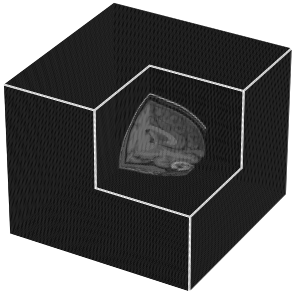
\includegraphics[height=3cm]{data/3d_bert.png}
                };
            }
            \visible<3-6>{
                \node[font=\fontsize{10}{10}\selectfont\bfseries, align=center] at (-1.75, 2) {
                    Structural Magnetic\\
                    Resonance Imaging (MRI) scans
                };

                \node[label=below:\small{Side}] (side) at (-3.5, -1.5) {
                    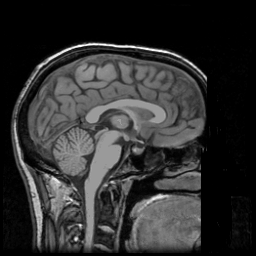
\includegraphics[height=3cm]{data/bert_x_enhanced.png}
                };

                \node[label=below:\small{Above}] at (0, -1.5) {
                    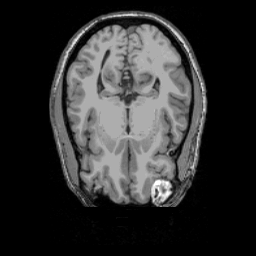
\includegraphics[height=3cm]{data/bert_y_enhanced.png}
                };

                \node[label=below:\small{Front}] at (3.5, -1.5) {
                    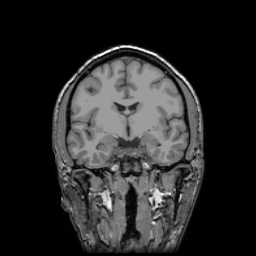
\includegraphics[height=3cm]{data/bert_z_enhanced.png}
                };
            }
            \visible<4-5>{
                \node[] at ($ (side.north east) + (0.5, 0.5) $) {
                    
\includegraphics[width=3cm]{data/region.png}
                };
                \node[
                    draw=red,
                    circle,
                    minimum size=3cm,
                    thick
                ] at ($ (side.north east) + (0.495, 0.495) $) {};
                \node[
                    draw=red,
                    circle,
                    minimum size=0.05cm,
                    inner sep=0pt,
                ] at ($ (side.north east) - (1.2, 1.12) $) {};
                \draw[red] ($ (side.north east) - (1.225, 1.12) $) --
                           ($ (side.north east) - (0.99, -0.75) $);
                \draw[red] ($ (side.north east) - (1.2, 1.145) $) --
                           ($ (side.north east) - (-0.75, 0.99) $);
            }
            \visible<5>{
                \node[
                    draw=red,
                    minimum height=0.6cm,
                    minimum width=0.6cm
                ] at ($ (side.north east) + (0.5, 0.5) $) {};

                \neuron{(0.1, 0.1)}{n0}
                \neuron{(0.05, 0.15)}{n1}
                \neuron{(-0.2, -0.1)}{n2}
                \neuron{(-0.15, 0.1)}{n3}
                \neuron{(0, -0.05)}{n4}
                \neuron{(0.13, -0.21)}{n5}
                \neuron{(0.15, -0.02)}{n6}
                \neuron{(-0.08, -0.13)}{n7}
                \neuron{(-0.05, 0.22)}{n8}

                \pgfplotsforeachungrouped  \i in {0,...,8} {
                    \pgfplotsforeachungrouped  \j in {0,...,8} {
                        \ifdim\i pt<\j pt
                            \draw[line width=0.25pt] (n\i) -- (n\j);
                        \fi
                    }
                }

                \neuron{(0.1, 0.1)}{n0}
                \neuron{(0.05, 0.15)}{n1}
                \neuron{(-0.2, -0.1)}{n2}
                \neuron{(-0.15, 0.1)}{n3}
                \neuron{(0, -0.05)}{n4}
                \neuron{(0.13, -0.21)}{n5}
                \neuron{(0.15, -0.02)}{n6}
                \neuron{(-0.08, -0.13)}{n7}
                \neuron{(-0.05, 0.22)}{n8}

            }
            \visible<6-7>{
                \node[rotate=-14] (label1) at ($ (threed) + (0.545, 1.46) $) {256};
                \node[rotate=37] (label2) at ($ (threed) + (-0.915, 1.3) $) {256};
                \node[rotate=93] (label3) at ($ (threed) - (1.67, 0.115) $) {256};
            }
            \visible<7>{
                \node[] (clinical) at (-3, 0) {
                    \usebox{\clinical}
                };
                \node[anchor=north, align=center, font=\small\selectfont\bfseries] at (clinical.south) {
                    Clinical datasets\\
                    ($n \approx 100$)
                };
            }
        \end{tikzpicture}
    \end{frame}

\end{document}
